\documentclass[10pt,openany]{book}
 
\usepackage{geometry, graphicx, varioref, soul, verbatim, amsmath, calc, caption, wasysym, footmisc, makeidx, ifthen, subfigure, multicol, epstopdf, enumerate, wrapfig, textcomp, multirow, changepage, setspace, lscape, titlesec}
\usepackage[usenames,dvipsnames]{color}  
%\newcommand{\href}[2]{#2} \newcommand{\url}[1]{#1} \newcommand{\urlstyle}[1]{}

\definecolor{oiGA}{rgb}{0,0,0}
\definecolor{oiGB}{rgb}{.5,.5,.5}
\definecolor{oiGC}{rgb}{.85,.85,.85}
%\definecolor{oiB}{rgb}{0.365,0.529,0.631}
\definecolor{oiB}{rgb}{.337,.608,.741}
%\definecolor{oiB}{rgb}{0,0,0}
\definecolor{oiG}{rgb}{.298,.447,.114}
\definecolor{oiY}{rgb}{.957,.863,0}
\definecolor{oiR}{rgb}{.941,.318,.200}
\definecolor{redcards}{rgb}{.941,.318,.200}


\definecolor{rd}{rgb}{.80,.0,.0}
\definecolor{tableHL}{rgb}{.5,.1,.2}
\definecolor{tableHLBlue}{rgb}{.2,.4,.9}
\definecolor{highlight}{rgb}{.5,.1,.2}
\definecolor{highlightO}{rgb}{.1,.3,.8}
\definecolor{highlightT}{rgb}{.6,.3,.1}
\definecolor{ex}{rgb}{.0,.30,.55}
\definecolor{gray}{rgb}{.5,.5,.5}
\definecolor{steelBlue}{rgb}{.3,.4,.8}
\definecolor{excolor}{rgb}{.0,.3,.55}
\definecolor{secolor}{rgb}{.0,.3,.55}
\definecolor{comment}{rgb}{.65,.45,.25}
\definecolor{grayDark}{rgb}{.43,.43,.43}
\definecolor{grayLight}{rgb}{.65,.65,.65}
\definecolor{examplegray}{rgb}{0,0,0} %{.83,.83,.83}
\definecolor{termOColor}{rgb}{.65,.1,.1}



% _____ Online Version _____ %
\usepackage[bookmarksnumbered, colorlinks = false, pdfborder = {0 0 0}, urlcolor = oiGB, colorlinks=true, linkcolor = oiGB, citecolor = oiGB, backref = true]{hyperref}
\newcommand{\versiondate}[0]{March 5th, 2016}

% _____ B&W Print Version _____ %
%\definecolor{oiB}{rgb}{0,0,0}\usepackage[colorlinks=false,pdfborder={0 0 0},urlcolor= black,colorlinks=black,linkcolor=black, citecolor=black,backref=true]{hyperref}

% _____ COLOR PRINT Version _____ %
%\usepackage[colorlinks=false,pdfborder={0 0 0},urlcolor= black,colorlinks=black,linkcolor=black, citecolor=black,backref=true]{hyperref}

\usepackage[style=authortitle-ibid, maxnames=2,natbib=true,sortcites=true,block=space,backend=bibtex]{biblatex}

\makeindex
% 1 Page Parameters
% 2 Special Commands for Editions
% 3 Content Modifications
% 4 Counters and Parameters
% 5 Section Coloring
% 6 Utilities
% 7 
% 8 Figures and Captions
% 9 Examples and Exercises
% 10 Special Boxes



%-------------------------------------------------------------
% 1 Page Parameters
% 1.1 Amazon
\setlength\paperheight{10in}
\setlength\textheight{8.25in}
\setlength\paperwidth{8in}
\setlength\textwidth{5.45in}
\setlength\voffset{-10mm}
% 1.2 Margin Size
% 1.2.1 Slim
%\setlength\hoffset{0.25in}
%\setlength\oddsidemargin{0.25in}
%\setlength\evensidemargin{0in}
% 1.2.2 Medium
\setlength\hoffset{3.7mm}
\setlength\oddsidemargin{3mm}
\setlength\evensidemargin{3mm}
% 1.2.3 Wide
%\setlength\hoffset{-5mm}
%\setlength\oddsidemargin{0.5in}
%\setlength\evensidemargin{0.5in}
% 1.3 PDF Parameters
%\setlength\paperheight{11in}
%\setlength\textheight{8.25in}
%\setlength\paperwidth{8.5in}
%\setlength\textwidth{5.45in}
%\setlength\voffset{-10mm}
%\setlength\oddsidemargin{0.75in}
%\setlength\evensidemargin{0.75in}
% 1.4 Margin Spacing
\setlength{\marginparsep}{5mm}
\setlength{\marginparwidth}{20mm}


% Tablet Version
%\setlength\paperheight{8.82in}\setlength\textheight{8.25in}\setlength\paperwidth{5.7in}\setlength\textwidth{5.45in}\setlength\voffset{-23.5mm}\setlength\hoffset{-27mm}\setlength\oddsidemargin{5mm}\setlength\evensidemargin{5mm}\setlength{\marginparsep}{5mm}\setlength{\marginparwidth}{35mm}




%-------------------------------------------------------------
% 2 Special Commands for Editions
\newcommand{\textA}[1]{#1}



%-------------------------------------------------------------
% 3 Content Modifications
\newcommand{\APVersion}[2]{#2}
\newcommand{\MultipleRegression}[2]{#1}
\newcommand{\MultipleRegressionChapter}[2]{#1}
\newcommand{\SimulationAndRandomization}[1]{#1}
\newcommand{\ANOVASection}[2]{#1}
\newcommand{\GLMSection}[2]{#1}




%-------------------------------------------------------------
% 4 Counters and Parameters
% 4.1 Counters
\newcounter{alwaysOne}
\setcounter{alwaysOne}{1}
\newcounter{alwaysTwo}
\setcounter{alwaysTwo}{2}
\newcounter{alwaysThree}
\setcounter{alwaysThree}{3}
\newcounter{alwaysFour}
\setcounter{alwaysFour}{4}
\newcounter{withinChNum}[chapter]
\setcounter{withinChNum}{0}
\newcounter{eoce}[chapter]
\renewcommand{\theeoce}{\arabic{chapter}.\arabic{eoce}}
\newcounter{eocesolch}
\setcounter{eocesolch}{0}
\newcounter{eocesol}[eocesolch]
% 4.2 Parameters
\newlength{\exampleAboveBar}
\newlength{\exampleBelowBar}
\setlength{\exampleAboveBar}{-3.15mm}
\setlength{\exampleBelowBar}{-1.15mm}
% 4.3 Chapter Declarations
\newcommand\includechapter[2]{
  \setcounter{chapter}{#1}
  \addtocounter{chapter}{-1}
  \normalsize
  \include{#2/TeX/#2}
  \include{#2/TeX/#2_ex}}



%-------------------------------------------------------------
% 5 Section Coloring
% 5.1 Chapter
\titleformat{\chapter}[display]
{\color{oiB}\normalfont\huge\bfseries\raggedright}{\chaptertitlename\
\thechapter}{20pt}{\Huge}
% 5.2 Section
\titleformat{\section}
{\color{oiB}\normalfont\Large\bfseries}
{\color{oiB}\thesection}{1em}{}
% 5.3 Subsection
\titleformat{\subsection}
{\color{oiB}\normalfont\large\bfseries}
{\color{oiB}\thesubsection}{1em}{}


%-------------------------------------------------------------
% 6 Utilities
% 6.1 Helpful Editing Commands
\newcommand\Add[1]{\marginpar[{\Huge\color{oiR}$\bullet$}]{\Huge\color{oiR}$\bullet$}{\color{oiB}#1}}
\newcommand\Cut[1]{\marginpar[{\Huge\color{oiR}$\bullet$}]{\Huge\color{oiR}$\bullet$}{\color{oiGC}#1}}
\newcommand\Comment[1]{\marginpar[{\Huge\color{oiR}$\bullet$}]{\Huge\color{oiR}$\bullet$} {\color{oiG}{[#1]}}}
\newcommand{\note}[1]{\Comment{#1}}
% 6.2 Special Symbols
\newcommand{\degree}{\ensuremath{^\circ}}
% 6.3 Text Commands (Terms, Data, Variable, Response)
\newcommand{\term}[1]{\textbf{#1}\index{#1|textbf}}
\newcommand{\termsub}[2]{\textbf{#1}\index{#2|textbf}}
\newcommand{\termni}[1]{\textbf{#1}}
\newcommand{\hiddenterm}[1]{#1\index{#1|textbf}}
\newcommand{\indexthis}[2]{#1\index{#2}}
\newcommand{\termO}[1]{\textbf{\color{termOColor}#1}}
\newenvironment{data}[1]{\texttt{#1}}{}
\newenvironment{var}[1]{\texttt{#1}}{}
\newenvironment{resp}[1]{\texttt{#1}}{}
\newenvironment{calctext}[1]{{\color{oiB}\texttt{#1}}}{}
\newenvironment{calctextmath}[1]{{\color{oiB}\mathtt{#1}}}{}
\newenvironment{calcbutton}[1]{{\color{oiB}\texttt{#1}}}{}
% 6.4 Highlighting
\newenvironment{highlight}{\textbf}{}
\newcommand{\highlightO}[1]{\textbf{\color{oiB}#1}}
\newcommand{\highlightT}[1]{\emph{\color{oiR}#1}}
% 6.5 Lengths
\setlength{\parindent}{0.3in}
% 6.6 Hyperreferences
\newcommand{\urlwofont}[1]{\urlstyle{same}\url{#1}}
\newcommand{\oiRedirect}[2]{\href{http://www.openintro.org/redirect.php?go=#1&referrer=ahss_pdf}{#2}}
\newcommand{\videohref}[2][4.5mm]{\oiRedirect{#2}{\raisebox{-0.3mm}[0pt]{
\includegraphics[height=#1]{extraTeX/icons/video_camera}}}}
\newcommand{\sectionvideohref}[2][6mm]{\oiRedirect{#2}{\raisebox{-0.5mm}[0pt]{
\includegraphics[height=#1]{extraTeX/icons/video_camera}}}}



%-------------------------------------------------------------
% 7 



%-------------------------------------------------------------
% 8 Figures and Captions
% 8.1 & 8.2 Table & Figure Numbering
% Thanks @Herbert on StackExchange for helping clean up this style code!
% http://tex.stackexchange.com/questions/176978/latex-numbering-in-counters-appears-to-have-changed/177045?noredirect=1#comment409945_177045
\makeatletter
\let\c@table\c@figure
\makeatother
% 8.3 Caption Width
\newlength{\mycaptionwidth}
\setlength{\mycaptionwidth}{0.825\textwidth}
\setlength{\captionwidth}{\mycaptionwidth}




%-------------------------------------------------------------
% 9 Examples and Exercises
% 9.1 Exercises, within the text
% 9.1.1 Exercise Environment
\newcommand{\excolor}[1]{{\color{excolor}#1}}
\newenvironment{exercise}
{
\begin{itemize}\item[\color{oiB}$\bigodot$]\refstepcounter{equation}\noindent\normalsize\textbf{\color{oiB}Guided Practice \theexercise}\hspace{3mm}}
{\normalsize

\addvspace{3mm}
\end{itemize}}
% 9.1.2 Exercise Fine Tuning
\newcommand\theexercise{\thechapter.\arabic{equation}}
% 9.2 Examples
% 9.2.1 Example Environment
\newcommand\theexample{\thechapter.\arabic{equation}}
\newenvironment{example}[1]
{\begin{itemize}
\item[\color{oiB}\Large$\CIRCLE$]\refstepcounter{equation}\noindent\textbf{\color{oiB}Example \theexample}\hspace{0.3cm}#1\vspace{\exampleAboveBar}

{\color{examplegray}\rule{20mm}{0.1mm}}

\vspace{\exampleBelowBar}

\normalsize}{

\end{itemize}
\addvspace{3mm}
}
% 9.3 EOCEs: End of Chapter Exercises
% 9.3.1 Environment
\newenvironment{eoce}[2]
{\refstepcounter{eoce}\noindent\small\textbf{\textcolor{oiB}{\arabic{chapter}.\arabic{eoce}}}\hspace{2mm} #1

\addvspace{3mm}

}
%{\em #2 } $\:$ \\ }
{}
% 9.3.2 EOCE Solutions
\newcommand{\eocesolch}[1]{
\refstepcounter{eocesolch}\noindent\textbf{\color{oiB}\arabic{eocesolch}\hspace{2mm}#1}

\addvspace{2mm}

}
\newcommand{\eocesol}[1]{\refstepcounter{eocesol}\noindent\textbf{\color{oiB}\arabic{eocesolch}.\arabic{eocesol}}\hspace{2mm}{\small#1}\addtocounter{eocesol}{1}

\addvspace{1mm}

}
% 9.3.3 EOCE Utilities
\newcommand{\qt}[1]{\textcolor{oiB}{\textbf{#1.}}}
\newcommand{\qtq}[1]{\textcolor{oiB}{\textbf{#1?}}}
\newcommand{\ec}[1]{\textcolor{oiB}{\footnotesize{~(#1)}}}% 9.3.4 EOCE Roman Parts
\newenvironment{romanparts}{
\begin{enumerate}[I.]
\setlength{\itemsep}{0mm}
}{\end{enumerate}}
% 9.3.5 EOCE Parts
\newenvironment{parts}{
%\vspace{-0.25cm}
\begin{enumerate}[(a)]
\setlength{\itemsep}{0mm}}
{\end{enumerate}}
% 9.3.6 EOCE Subparts
\newenvironment{subparts}{
\begin{enumerate}[i.]
\setlength{\itemsep}{0mm}}
{\end{enumerate}}
% 9.3.7 EOCE hyp environment
\newenvironment{hyp}{
\begin{itemize}
\setlength{\itemsep}{0mm}
}
{\end{itemize}
}
% 9.3.8 cond environment
\newenvironment{cond}{
\begin{enumerate}[1.]
\setlength{\itemsep}{0mm}
}
{\end{enumerate}
}




%-------------------------------------------------------------
% 10 Special Boxes
% 10.1 Term Box
\newcommand\tBoxTitleBuffer{\\[1.5mm]}
\newenvironment{tBoxTitle}[2][\tBoxTitleBuffer]{\textbf{\color{oiB}#2} #1
}{}
\newenvironment{termBox}[1]{
\addvspace{4mm}
\noindent{\color{oiB}\framebox[\textwidth][c]{\framebox[\textwidth-3mm][l]{ \\
	\vspace{0.5cm} \\
	\begin{minipage}[b]{\textwidth-3mm}
		\begin{minipage}[t]{2mm}
			\hspace{2mm}
		\end{minipage}
		\begin{minipage}[b]{\textwidth-10mm}
			\color{black}\ 
			
			#1
			
			\vspace{1.5mm}
		\end{minipage}
	\end{minipage}}}}
}{

\addvspace{1mm}}
% 10.2 Tip Box
\newenvironment{tipBoxTitle}[2][TIP:\ ]{\textbf{\color{oiB}#1#2} \\
}{}
\newenvironment{tipBox}[1]{
\addvspace{4mm}
\noindent{\color{oiB}\framebox[\textwidth][l]{ \\
	\vspace{5mm} \\
	\begin{minipage}[b]{\textwidth-4mm}
		\begin{minipage}[t]{2mm}
			\hspace{2mm}
		\end{minipage}
		\begin{minipage}[b]{\textwidth-8mm}
			\color{black}\ 
			
			#1
			
			\vspace{1.5mm}
		\end{minipage}
	\end{minipage}}}
}{

\addvspace{1mm}}
% 10.3 Caution Box
\newenvironment{caution}[2]{
\addvspace{4mm}
\noindent{\color{oiB}\framebox[\textwidth][l]{ \\
	\vspace{5mm} \\
	\begin{minipage}[b]{\textwidth-4mm}
		\begin{minipage}[t]{2mm}
			\hspace{2mm}
		\end{minipage}
		\begin{minipage}[b]{\textwidth-8mm}
			\textbf{\color{oiB}Caution: #1} \\
			\color{black}#2
		\end{minipage}
	\end{minipage}}}
}{

\addvspace{1mm}}







%
% Tablet Version
\setlength\paperheight{8.82in}
\setlength\textheight{8.25in}
\setlength\paperwidth{5.7in}
\setlength\textwidth{5.45in}
\setlength\voffset{-23.5mm}
\setlength\hoffset{-27mm}
\setlength\oddsidemargin{5mm}
\setlength\evensidemargin{5mm}
\setlength{\marginparsep}{5mm}
\setlength{\marginparwidth}{35mm}



\title{\huge TI-83/84 Guide for Introductory Statistics\vspace{10mm} \\ \Large Includes step-by-step instructions, \\practice exercises, and links to video \\tutorials.  Covers all calculator features \\needed for AP\textregistered{}  Statistics Exam \vspace{10mm} \\ \Large Instructions excerpted from \\ \emph{Advanced High School Statistics}, \\available for FREE at \href{https://www.openintro.org/stat/textbook.php?stat_book=aps}{openintro.org} \vspace{20mm}}
\author{
Leah Dorazio \\
\small\emph{San Francisco University High School} \\
\small\emph{leah@openintro.org}}

\usepackage{geometry}

\usepackage{remreset}

\makeatletter
  \renewcommand \thesection {\@arabic\c@section}
  \@removefromreset{section}{chapter}
\makeatother
\setcounter{tocdepth}{1}


\begin{document}





\maketitle

\chapter*{}
\vfill

\noindent Copyright $\copyright$ 2016 OpenIntro, Inc. \\
Updated: \today. \\

\noindent This guide is available under a Creative Commons license. % Attribution-ShareAlike license. \\
Visit \oiRedirect{openintro.org}{openintro.org} for a free PDF, to download the source files, or for more information about the license. \\

%\noindent Modified versions of this textbook, including reformatted electronic versions, may not be redistributed under a title that suggests association with or endorsement by OpenIntro, e.g. it cannot be titled \emph{OpenIntro Statistics}. %More information on branding restrictions for derivatives is available on the Rights page at~\href{http://www.openintro.org/rights.php}{openintro.org}.

\noindent {\scriptsize AP\textregistered{} is a trademark registered and owned by the College Board, which was not involved in the production of, and does not endorse, this product.}




\tableofcontents

\chapter*{Summarizing data}
\addcontentsline{toc}{chapter}{ Summarizing data}


\section*{Entering data}
\addcontentsline{toc}{section}{Entering data}

\begin{termBox}{\tBoxTitle{\videohref{ti84_entering_data} TI-83/84: Entering data}
The first step in summarizing data or making a graph is to  enter the data set into a list. Use \calcbutton{STAT}, \calctext{Edit}.
\begin{enumerate}
\setlength{\itemsep}{0mm}
\item Press \calcbutton{STAT}.
\item Choose \calctext{1:Edit}.
\item Enter data into \calctext{L1} or another list.
\end{enumerate}
}
\end{termBox}

\section*{Calculating summary statistics}
\addcontentsline{toc}{section}{Calculating summary statistics}

\begin{termBox}{\tBoxTitle{\videohref{ti84_calculating_summary_statistics} TI-84: Calculating Summary Statistics}
Use the \calcbutton{STAT}, \calctext{CALC}, \calctext{1-Var Stats} command to find summary statistics such as mean, standard deviation, and quartiles.
\begin{enumerate}
\setlength{\itemsep}{0mm}
\item Enter the data as described previously.
\item Press \calcbutton{STAT}.
\item Right arrow to \calctext{CALC}.
\item Choose \calctext{1:1-Var Stats}.
\item Enter \calctext{L1} (i.e. \calcbutton{2ND} \calcbutton{1}) for List. If the data is in a list other than \calctext{L1}, type the name of that list.
\item Leave \calctext{FreqList} blank.
\item Choose \calctext{Calculate} and hit \calcbutton{ENTER}.
\end{enumerate}
TI-83: Do steps 1-4, then type \calctext{L1} (i.e. \calcbutton{2nd} \calcbutton{1}) or the list's name and hit \calcbutton{ENTER}.
}
\end{termBox}

\newpage

Calculating the summary statistics will return the following information. It will be necessary to hit the down arrow to see all of the summary statistics.

\begin{center}
\begin{tabular}{ll l ll}
$\calctextmath{\bar{\text{x}}}$ & Mean &\quad&
	\calctext{minX} & Minimum \\
$\calctextmath{\Sigma x}$ & Sum of all the data values &&
	$\calctextmath{Q_1}$ & First quartile \\
$\calctextmath{\Sigma x^2}$ & Sum of all the squared data values &&
	\calctext{Med} & Median\\
$\calctextmath{\sigma x}$ & Population standard deviation &&
	\calctext{maxX} & Maximum \\
\calctext{n} & Sample size or \# of data points
\end{tabular}
\end{center}

\section*{Drawing a box plot}
\addcontentsline{toc}{section}{Drawing a box plot}

\begin{termBox}{\tBoxTitle{\videohref{ti84_box_plot} TI-83/84:  Drawing a box plot}
\begin{enumerate}
\setlength{\itemsep}{0mm}
\item Enter the data to be graphed as described previously.
\item Hit \calcbutton{2ND} \calcbutton{Y=} (i.e. \calctext{STAT PLOT}).
\item Hit \calcbutton{ENTER} (to choose the first plot).
\item Hit \calcbutton{ENTER} to choose \calctext{ON}.
\item Down arrow and then right arrow three times to select box plot with outliers.
\item Down arrow again and make \calctext{Xlist:}~\calctext{L1} and \calctext{Freq:}~\calctext{1}.
\item Choose \calctext{ZOOM} and then \calctext{9:ZoomStat} to get a good viewing window.
\end{enumerate}
}
\end{termBox}

\section*{What to do if you cannot find L1 or another list}
\addcontentsline{toc}{section}{What to do if you cannot find L1 or another list}

\begin{tipBox}{\tBoxTitle{TI-83/84: What to do if you cannot find \calctext{L1} or another list}
Restore lists \calctext{L1}-\calctext{L6} using the following steps:
\begin{enumerate}
\setlength{\itemsep}{0mm}
\item Press \calcbutton{STAT}.
\item Choose \calctext{5:SetUpEditor}.
\item Hit \calcbutton{ENTER}.
\end{enumerate}}
\end{tipBox}

\newpage

\section*{Practice exercises}
\addcontentsline{toc}{section}{Practice exercises}

\begin{exercise}Enter the following 10 data points into the first list on a calculator: {5, 8, 1, 19, 3, 1, 11, 18, 20, 5}. Find the summary statistics and make a box plot of the data.
The summary statistics should be $\calctextmath{\bar{x}} = 9.1$, $\calctextmath{Sx} = 7.475$, $\calctextmath{Q1} = 3$, etc. The box plot should be as follows.
\begin{center}
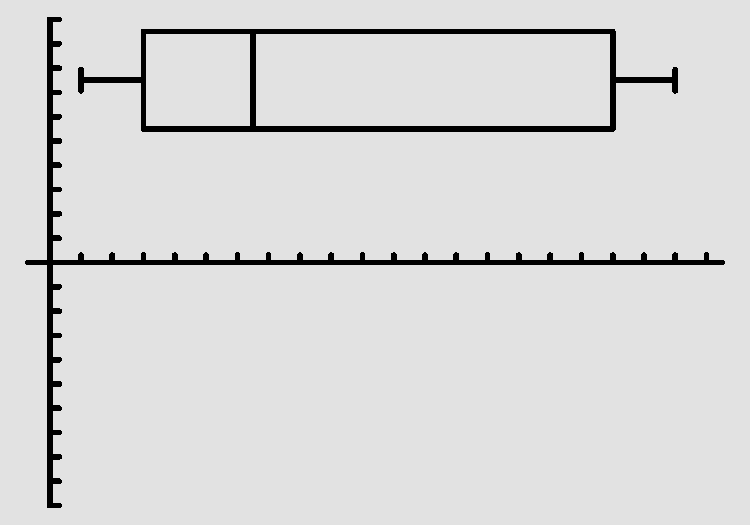
\includegraphics[width=0.45\textwidth]{ch_summarizing_data/figures/TI83_box_plot_A/TI83_box_plot_A}
\end{center}
\end{exercise}


\chapter*{Probability}
\addcontentsline{toc}{chapter}{Probability}

\section*{Computing the binomial coefficient}
\addcontentsline{toc}{section}{Computing the binomial coefficient}



\begin{termBox}{\tBoxTitle{\videohref{ti84_binomial_coefficient} TI-83/84: Computing the binomial coefficient, ${n\choose k}$}
Use \calctext{MATH}, \calctext{PRB}, \calctext{nCr} to evaluate $n$ choose $r$. Here $r$ and $k$ are different letters for the same quantity.
\begin{enumerate}
\setlength{\itemsep}{0mm}
\item Type the value of n.
\item Select \calctext{MATH}.
\item Right arrow to \calctext{PRB}.
\item Choose \calctext{3:nCr}.
\item Type the value of k.
\item Hit \calcbutton{ENTER}.
\end{enumerate}
Example: \calctext{5 nCr 3} means \emph{5 choose 3}.}
\end{termBox}

\newpage

\section*{Computing the binomial formula}
\addcontentsline{toc}{section}{Computing the binomial formula}

\begin{termBox}{\tBoxTitle{\videohref{ti84_binomial_formula} TI-84: Computing the binomial formula, $P(X = k)={n\choose k}p^k(1-p)^{n-k}$}
Use \calcbutton{2ND} \calcbutton{VARS}, \calctext{binompdf} to evaluate the probability of \emph{exactly} $k$ occurrences out of $n$ independent trials of an event with probability $p$. 
\begin{enumerate}
\setlength{\itemsep}{0mm}
\item Select \calcbutton{2ND} \calcbutton{VARS} (i.e. \calctext{DISTR})
\item Choose \calctext{A:binompdf} (use the down arrow).
\item Let \calctext{trials} be $n$.
\item Let \calctext{p} be $p$
\item Let \calctext{x} value be $k$.
\item Select \calctext{Paste} and hit \calcbutton{ENTER}.\vspace{-1.5mm}
\end{enumerate}
TI-83: Do steps 1-2, then enter $n$, $p$, and $k$ separated by commas:\\
	\calctext{binompdf(n,~p,~k)}. Then hit \calcbutton{ENTER}. 
}
\end{termBox}

\section*{Computing a cumulative binomial probability}
\addcontentsline{toc}{section}{Computing a cumulative binomial probability}

\begin{termBox}{\tBoxTitle{\videohref{ti84_binomial_cdf} TI-84: Computing $P(X \le k)= {n\choose 0}p^0(1-p)^{n-0} + ... + {n\choose k}p^k(1-p)^{n-k}$} 
Use \calcbutton{2ND} \calcbutton{VARS}, \calctext{binomcdf} to evaluate the cumulative probability of \emph{at most} $k$ occurrences out of $n$ independent trials of an event with probability $p$. 
\begin{enumerate}
\setlength{\itemsep}{0mm}
\item Select \calcbutton{2ND} \calcbutton{VARS} (i.e. \calctext{DISTR})
\item Choose \calctext{B:binomcdf} (use the down arrow).
\item Let \calctext{trials} be $n$.
\item Let \calctext{p} be $p$
\item Let \calctext{x} value be $k$.
\item Select \calctext{Paste} and hit \calcbutton{ENTER}.\vspace{-1.5mm}
\end{enumerate}
TI-83: Do steps 1-2, then enter the values for $n$, $p$, and $k$ separated by commas as follows: \calctext{binomcdf(n,~p,~k)}. Then hit \calctext{ENTER}.}
\end{termBox}

\newpage

\section*{Practice exercises}
\addcontentsline{toc}{section}{Practice exercises}

\begin{exercise}
Find the number of ways of arranging 3 blue marbles and 2 red marbles.\footnote{Use $n$ = 5 and $k$ = 3 to get 10.}
\end{exercise}

\begin{exercise}There are 13 marbles in a bag. 4 are blue and 9 are red. Randomly draw 5 marbles \emph{with replacement}. Find the probability you get exactly 3 blue marbles.\footnote{Use $n$ = 5, $p$ = 4/13, and $x$ ($k$) = 3 to get 0.1396.}
\end{exercise}

\begin{exercise}There are 13 marbles in a bag. 4 are blue and 9 are red. Randomly draw 5 marbles \emph{with replacement}. Find the probability you get \emph{at most} 3 blue marbles (i.e. less than or equal to 3 blue marbles).\footnote{Use $n = 5$, $p = 4/13$, and $x = 3$ to get 0.9662.}
\end{exercise}

\newpage

\chapter*{Distribution of random variables}
\addcontentsline{toc}{chapter}{Distribution of random variables}


\section*{Finding area under the normal curve}
\addcontentsline{toc}{section}{Finding area under the normal curve}

\begin{termBox}{\tBoxTitle{\videohref{ti84_normal_curve_area} TI-84: Finding area under the normal curve}
Use \calcbutton{2ND} \calcbutton{VARS}, \calctext{normalcdf} to find an area/proportion/probability to the left or right of a Z-score or between two Z-scores.\vspace{-1mm}
\begin{enumerate}
\setlength{\itemsep}{0mm}
\item Choose \calcbutton{2ND} \calcbutton{VARS} (i.e. \calctext{DISTR}).
\item Choose \calctext{2:normalcdf}.
\item Enter the Z-scores that correspond to the lower (left) and upper (right) bounds.
\item Leave $\calctextmath{\mu}$ as \calctext{0} and $\calctextmath{\sigma}$ as \calctext{1}.
\item Down arrow, choose \calctext{Paste}, and hit \calcbutton{ENTER}.\vspace{-1.5mm}
\end{enumerate}
TI-83: Do steps 1-2, then enter the lower bound and upper bound separated by a comma, e.g. \calctext{normalcdf(2, 5)}, and hit \calcbutton{ENTER}.}
\end{termBox}

\newpage

\section*{Find a Z-score that corresponds to a percentile}
\addcontentsline{toc}{section}{Find a Z-score that corresponds to a percentile}

\begin{termBox}{\tBoxTitle{\videohref{ti84_Z_score_for_a_percentile} TI-84: Find a Z-score that corresponds to a percentile}
Use \calcbutton{2ND} \calcbutton{VARS}, \calctext{invNorm} to find the Z-score that corresponds to a given percentile.
\begin{enumerate}
\setlength{\itemsep}{0mm}
\item Choose \calcbutton{2ND} \calcbutton{VARS} (i.e. \calctext{DISTR}).
\item Choose \calctext{3:invNorm}.
\item Let \calctext{Area} be the percentile as a decimal (the area to the left of desired Z-score).
\item Leave $\calctextmath{\mu}$ as \calctext{0} and $\calctextmath{\sigma}$ as \calctext{1}.
\item Down arrow, choose \calctext{Paste}, and hit \calcbutton{ENTER}.\vspace{-1.5mm}
\end{enumerate}
TI-83: Do steps 1-2, then enter the percentile as a decimal, e.g.~\mbox{\calctext{invNorm(.40)},} then hit \calcbutton{ENTER}.}
\end{termBox}

\newpage

\section*{Practice exercises}
\addcontentsline{toc}{section}{Practice exercises}

\begin{example}{Use a calculator to determine what percentile corresponds to a Z-score of 1.5.}
Always first sketch a graph:\footnote{normalcdf gives the result without drawing the graph. To draw the graph, do 2nd VARS, DRAW, 1:ShadeNorm. However, beware of errors caused by other plots that might interfere with this plot.}
\begin{center}
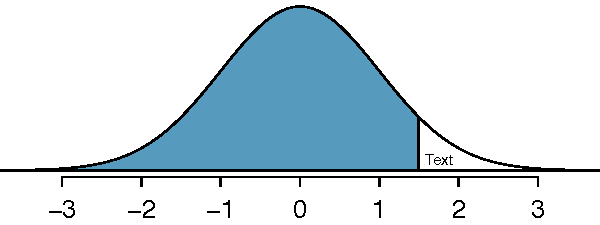
\includegraphics[width=0.57\textwidth]{ch_distributions/figures/zscoreleftof1point5/zscoreleftof1point5}\vspace{-2mm}
\end{center}
To find an area under the normal curve using a calculator, first identify a lower bound and an upper bound. Theoretically, we want all of the area to the left of 1.5, so the left endpoint should be -$\infty$. However, the area under the curve is nearly negligible when $Z$ is smaller than -4, so we will use -5 as the lower bound when not given a lower bound (any other negative number smaller than -5 will also work). Using a lower bound of -5 and an upper bound of 1.5, we get $P(Z < 1.5) = 0.933$.
\end{example}

\begin{exercise}
Find the area under the normal curve to right of $Z=2$.~\footnote{Now we want to shade to the right. Therefore our lower bound will be 2 and the upper bound will be +5 (or a number bigger than 5) to get $P(Z > 2) = 0.023$.}
\end{exercise}

\begin{exercise}Find the area under the normal curve between -1.5 and~1.5.~\footnote{Here we are given both the lower and the upper bound. Lower bound is -1.5 and upper bound is 1.5. The area under the normal curve between -1.5 and 1.5 = $P(-1.5 < Z < 1.5) = 0.866$.}
\end{exercise}


\begin{example}{Use a calculator to find the Z-score that corresponds to the 40th percentile.}Letting Area be 0.40, a calculator gives -0.253. This means that $Z = -0.253$ corresponds to the 40th percentile, that~is, $P(Z < -0.253) = 0.40$.
\end{example}

\begin{exercise}Find the Z-score such that 20 percent of the area is to the right of that Z-score.\footnote{If 20\% of the area is the right, then 80\% of the area is to the left. Letting area be 0.80, we get $Z = 0.841$.}
\end{exercise}	


\chapter*{Inference for categorical data}
\addcontentsline{toc}{chapter}{Inference for categorical data}

\section*{1-proportion $z$-interval and $z$-test}
\addcontentsline{toc}{section}{1-proportion $z$-interval and $z$-test}

\begin{termBox}{\tBoxTitle{\videohref{ti84_1_prop_CI} TI-83/84: 1-proportion $z$-interval}
Use \calcbutton{STAT}, \calctext{TESTS}, \calctext{1-PropZInt}.
\begin{enumerate}
\setlength{\itemsep}{0mm}
\item Choose \calcbutton{STAT}.
\item Right arrow to \calctext{TESTS}.
\item Down arrow and choose \calctext{A:1-PropZInt}.
\item Let \calctext{x} be the \emph{number} of yes's (must be an integer).
\item Let \calctext{n} be the sample size.
\item Let \calctext{C-Level} be the desired confidence level.
\item Choose \calctext{Calculate} and hit \calcbutton{ENTER}, which returns\\[1mm]
\begin{tabular}{l l}
\calctext{(\underline{\ \ },\underline{\ \ })} & the confidence interval \\
$\calctextmath{\hat{p}}$ & the sample proportion \\
\calctext{n} & the sample size
\end{tabular}
\end{enumerate}
}
\end{termBox}

\newpage

\begin{termBox}{\tBoxTitle{\videohref{ti84_1_prop_HT} TI-83/84: 1-proportion $z$-test}
Use \calcbutton{STAT}, \calctext{TESTS}, \calctext{1-PropZTest}.
\begin{enumerate}
\setlength{\itemsep}{0mm}
\item Choose \calcbutton{STAT}.
\item Right arrow to \calctext{TESTS}.
\item Down arrow and choose \calctext{5:1-PropZTest}.
\item Let $\calctextmath{p_0}$ be the null or hypothesized value of p.
\item Let \calctext{x} be the \emph{number} of yes's (must be an integer).
\item Let \calctext{n} be the sample size.
\item Choose $\calctextmath{\ne}$, $\calctextmath{<}$, or $\calctextmath{>}$ to correspond to H$_A$.
\item Choose \calctext{Calculate} and hit \calcbutton{ENTER}, which returns \\[1mm]
\begin{tabular}{l l}
\calctext{z} & Z-statistic \\
\calctext{p} & p-value \\
$\calctextmath{\hat{p}}$ &  the sample proportion \\
\calctext{n} & the sample size
\end{tabular}
\end{enumerate}
}
\end{termBox}


\section*{Practice exercises}
\addcontentsline{toc}{section}{Practice exercises}

\begin{exercise}
A candidate selects a random sample of size $n=500$.  The proportion of people in the sample that support her is 52\%.  Is there significant evidence that greater than 50\% of the population support her?  Use a calculator to find the p-value for a test with  H$_A: p >$ 50\%.~\footnote{p-value = 0.19}
\end{exercise}

\begin{exercise}
What percent of Americans believe the Supreme Court is doing a good job?  A random sample of  $n = 976$ yields a sample percent of 44\%.  Use a calculator to find a 90\% confidence interval for the percent of all Americans that believe the Supreme Court is doing a good job.~\footnote{The interval is (0.414, 0.471) =  (41.4\%, 47.1\%). }
\end{exercise}

\section*{2-proportion $z$-interval and $z$-test}
\addcontentsline{toc}{section}{2-proportion $z$-interval and $z$-test}

\begin{termBox}{\tBoxTitle{\videohref{ti84_2_prop_CI} TI-83/84: 2-proportion $z$-interval}
Use \calcbutton{STAT}, \calctext{TESTS}, \calctext{2-PropZInt}.
\begin{enumerate}
\setlength{\itemsep}{0mm}
\item Choose \calcbutton{STAT}.
\item Right arrow to \calctext{TESTS}.
\item Down arrow and choose \calctext{B:2-PropZInt}.
\item Let \calctext{x1} be the \emph{number} of yes's (must be an integer) in sample 1 and let \calctext{n1} be the size of sample 1.
\item Let \calctext{x2} be the \emph{number} of yes's (must be an integer) in sample 2 and let \calctext{n2} be the size of sample 2.
\item Let \calctext{C-Level} be the desired confidence level.
\item Choose \calctext{Calculate} and hit \calcbutton{ENTER}, which returns: \\
\begin{tabular}{ll l ll}
\calctext{(\underline{\ \ },\underline{\ \ })} & the confidence interval \\
$\calctextmath{\hat{p}_1}$ & sample 1 proportion &\quad&
	$\calctextmath{n_1}$ & size of sample 1 \\
$\calctextmath{\hat{p}_2}$ & sample 2 proportion &&
	$\calctextmath{n_2}$ &  size of sample 2
\end{tabular}
\end{enumerate}
}
\end{termBox}

\begin{termBox}{\tBoxTitle{\videohref{ti84_2_prop_HT} TI-83/84: 2-proportion $z$-test}
Use \calcbutton{STAT}, \calctext{TESTS}, \calctext{2-PropZTest}.
\begin{enumerate}
\setlength{\itemsep}{0mm}
\item Choose \calcbutton{STAT}.
\item Right arrow to \calctext{TESTS}.
\item Down arrow and choose \calctext{6:2-PropZTest}.
\item Let \calctext{x1} be the \emph{number} of yes's (must be an integer) in sample 1 and let \calctext{n1} be the size of sample 1.
\item Let \calctext{x2} be the \emph{number} of yes's (must be an integer) in sample 2 and let \calctext{n2} be the size of sample 2.
\item Choose $\calctextmath{\ne}$, $\calctextmath{<}$, or $\calctextmath{>}$ to correspond to H$_A$.
\item Choose \calctext{Calculate} and hit \calcbutton{ENTER}, which returns:\\
\begin{tabular}{ll l ll}
\calctext{z} & Z-statistic &\quad&
	\calctext{p} & p-value \\
$\calctextmath{\hat{p}_1}$ & sample 1 proportion &&
	$\calctextmath{\hat{p}}$ & pooled sample proportion \\
$\calctextmath{\hat{p}_2}$ & sample 2 proportion
\end{tabular}
\end{enumerate}}
\end{termBox}

\newpage

\section*{Practice exercises}
\addcontentsline{toc}{section}{Practice exercises}

\begin{exercise}{Use the data in Table~\ref{24DAndCancerInDogsTableInCalcSection} and a calculator to find a 95\% confidence interval for the difference in proportion of dogs with cancer that have been exposed to 2,4-D versus not exposed to 2,4-D.}\footnote{Correctly going through the calculator steps should lead to an interval of (0.01484, 0.11926). There is no value given for the pooled proportion since we do not pool for confidence intervals.}
\end{exercise}

\begin{table}[h]
\centering
\begin{tabular}{rrr}
  \hline
 & cancer & no cancer \\
  \hline
2,4-D & 191 & 304 \\
no 2,4-D & 300 & 641 \\
   \hline
\end{tabular}
\caption{Summary results for cancer in dogs and the use of 2,4-D by the dog's owner.}
\label{24DAndCancerInDogsTableInCalcSection}
\end{table}


\begin{exercise}{Use the data in Table~\ref{24DAndCancerInDogsTableInCalcSection} and a calculator to find the Z-score and p-value for one-sided test with H$_A$: dogs with cancer are more likely to have been exposed to 2,4-D than dogs without cancer, $p_c - p_n > 0$.}\footnote{Correctly going through the calculator steps should lead to a solution with $Z=2.55$ and $\text{p-value}=0.0055$. The pooled proportion is $\hat{p}=0.342$.}
\end{exercise}

\newpage

\section*{Finding areas under the Chi-square curve}
\addcontentsline{toc}{section}{Finding area unders the Chi-square curve}

\begin{termBox}{\tBoxTitle{\videohref{ti84_chisq_tail_area} TI-84: Finding an upper tail area under the chi-square curve}
Use the $\calctextmath{X^2}$\calctext{cdf} command to find areas under the chi-square curve.
\begin{enumerate}
\setlength{\itemsep}{0mm}
\item Hit \calcbutton{2ND} \calcbutton{VARS} (i.e. \calctext{DISTR}).
\item Choose \calctext{8:}$\calctextmath{X^2}$\calctext{cdf}.
\item Enter the lower bound, which is generally the chi-square value.
\item Enter the upper bound. Use a large number, such as 1000.
\item Enter the degrees of freedom.
\item Choose \calctext{Paste} and hit \calcbutton{ENTER}.
\end{enumerate}
TI-83: Do steps~1-2, then type the lower bound, upper bound, and degrees of freedom separated by commas. e.g. $\calctextmath{X^2}$\calctext{cdf(5, 1000, 3)}, and hit \calcbutton{ENTER}.}
\end{termBox}

\section*{Chi-square goodness of fit test}
\addcontentsline{toc}{section}{Chi-square goodness of fit test}

\begin{termBox}{\tBoxTitle{\videohref{ti84_chisq_GOF_test} TI-84: Chi-square goodness of fit test\vspace{0.5mm}}
Use \calctext{STAT}, \calctext{TESTS}, $\calctextmath{X^2}$\calctext{GOF-Test}.
\begin{enumerate}
\setlength{\itemsep}{0mm}
\item Enter the observed counts into list \calctext{L1} and the expected counts into list \calctext{L2}.
\item Choose \calctext{STAT}.
\item Right arrow to \calctext{TESTS}.
\item Down arrow and choose \calctext{D:}$\calctextmath{X^2}$\calctext{GOF-Test}.
\item Leave \calctext{Observed:~L1} and \calctext{Expected:~L2}.
\item Enter the degrees of freedom after \calctext{df}:
\item Choose \calctext{Calculate} and hit \calcbutton{ENTER}, which returns: \\[1mm]
\begin{tabular}{l ll}
$\calctextmath{X^2}$ & chi-square test statistic \\
\calctext{p} & p-value \\
\calctext{df} & degrees of freedom
\end{tabular}
\end{enumerate}
TI-83: Unfortunately the TI-83 does not have this test built in. To carry out the test manually, make list \calctext{L3 = (L1 - L2)}$\calctextmath{^2}$\calctext{ / L2} and do \calctext{1-Var-Stats} on \calctext{L3}. The sum of \calctext{L3} will correspond to the value of $X^2$ for this test.}
\end{termBox}

\section*{Chi-square test for two-way tables}
\addcontentsline{toc}{section}{Chi-square test for two-way tables}

\begin{termBox}{\tBoxTitle[]{\videohref{ti84_chisq_2_way_test} TI-83/84: Entering data into a two-way table}
\begin{enumerate}
\setlength{\itemsep}{0mm}
\item Hit \calcbutton{2ND} $\calctextmath{x^{-1}}$ (i.e. \calctext{MATRIX}).
\item Right arrow to \calctext{EDIT}.
\item Hit \calcbutton{1} or \calcbutton{ENTER} to select matrix \calctext{A}.
\item Enter the dimensions by typing \#rows, \calcbutton{ENTER}, \#columns, \calcbutton{ENTER}.
\item Enter the data from the two-way table.
\end{enumerate}
}
\end{termBox}

\begin{termBox}{\tBoxTitle{\videohref{ti84_chisq_2_way_test} TI-83/84: Chi-square test of homogeneity and independence}
Use \calctext{STAT}, \calctext{TESTS}, $\calctextmath{X^2}$\calctext{-Test}.
\begin{enumerate}
\setlength{\itemsep}{0mm}
\item First enter two-way table data as described in the previous box.
\item Choose \calctext{STAT}.
\item Right arrow to \calctext{TESTS}.
\item Down arrow and choose \calctext{C:}$\calctextmath{X^2}$\calctext{-Test}.
\item Down arrow, choose \calctext{Calculate}, and hit \calcbutton{ENTER}, which returns \\[1mm]
\begin{tabular}{l l}
$\calctextmath{X^2}$ & chi-square test statistic \\
\calctext{p} & p-value \\
\calctext{df} & degrees of freedom
\end{tabular}
\end{enumerate}
}
\end{termBox}


\begin{termBox}{\tBoxTitle[]{TI-83/84: Finding the expected counts}
\begin{enumerate}
\setlength{\itemsep}{0mm}
\item First enter two-way table data as described previously.
\item Carry out the chi-square test of homogeneity or independence as described in previous box.
\item Hit \calctext{2ND} $\calctextmath{x^{-1}}$ (i.e. \calctext{MATRIX}).
\item Right arrow to \calctext{EDIT}.
\item Hit \calcbutton{2} to see matrix \calctext{B}.
\begin{description}
\item[] This matrix contains the expected counts.
\end{description}
\end{enumerate}
}
\end{termBox}


\section*{Practice exercises}
\addcontentsline{toc}{section}{Practice exercises}

\begin{exercise}
Use a calculator to find the area to right of 5.1 for a chi-square distribution with 5 degrees of freedom, i.e. find the upper tail area using a cutoff of 5.1. ~\footnote{Using $df = 5$ and a \emph{lower} bound of $5.1$ for the tail, the upper tail area is 0.4038.}
\end{exercise}


\begin{exercise}
Use the table below and a calculator to find the $X^2$ statistic, df, and p-value for chi-square goodness of fit test.~\footnote{You should find that $X^2=15.08$, $df=6$, and $\text{p-value}=0.0196$.}
\end{exercise}

\begin{table}[h]
\centering
\begin{tabular}{ll ccc ccc c ll}
\hline
Days	 & \hspace{1mm} & 1 & 2 & 3 & 4 & 5 & 6 & 7+ & \hspace{1mm} & Total \\
\hline
Observed values&		& 1532 & 760 & 338 & 194 & 74 & 33 & 17 & & 2948 \\
Expected values &  & 1569 & 734 & 343 & 161 & 75 & 35 & 31 & & 2948 \\
\hline
\end{tabular}
\caption{Distribution of the waiting time until a positive trading day. The expected counts are based on a geometric model.}
\end{table}


\begin{exercise}
Use the table below and a calculator to find the expected values and the $X^2$ statistic, $df$, and p-value for the corresponding chi-square test.~\footnote{First create a $2\times 3$ matrix ith the data. The final summaries should be $X^2=106.4$, $\text{\mbox{p-value}} = 8.06 \times 10^{-24}\approx 0$, and $df=2$. Below is the matrix of expected values:
\begin{center}
\begin{tabular}{l ccc}
&Obama  &Congr. Dem. & Congr. Rep. \\
\hline
Approve				    & 731.59    & 693.45 & 693.96   \\
Disapprove			    & 726.41    & 688.55 & 689.04  \\
\hline
\end{tabular}
\end{center}
}
\end{exercise}


\begin{table}[h]
\centering
\begin{tabular}{ll ccc ll}
& & & \multicolumn{2}{c}{Congress} & \\
\cline{4-5}
 & \hspace{1mm} & Obama & Democrats & Republicans & \hspace{1mm} & Total \\
\hline
Approve				   & & 842    & 736 & 541   & 				& 2119 \\
Disapprove			   & & 616    & 646 & 842   &				& 2104 \\
\hline
Total					   & & 1458    & 1382 & 1383 & 				& 4223 \\
\hline
\end{tabular}
\caption{Pew Research poll results of a March 2012 poll.}
\end{table}


\chapter*{Inference for numerical data}
\addcontentsline{toc}{chapter}{Inference for numerical data}


\section*{1-sample $t$-test and $t$-interval}
\addcontentsline{toc}{section}{1-sample $t$-test and $t$-interval}


\begin{termBox}{\tBoxTitle{\videohref{ti84_1_mean_HT} TI-83/84: 1-sample $t$-test}
Use \calctext{STAT}, \calctext{TESTS}, \calctext{T-Test}.
\begin{enumerate}
\setlength{\itemsep}{0mm}
\item Choose \calcbutton{STAT}.
\item Right arrow to \calctext{TESTS}.
\item Down arrow and choose \calctext{2:T-Test}.
\item Choose \calctext{Data} if you have all the data or \calctext{Stats} if you have the mean and standard deviation.
\item Let $\mu_0$ be the null or hypothesized value of $\mu$.
\begin{itemize}
\item If you choose \calctext{Data}, let \calctext{List} be \calctext{L1} or the list in which you entered your data (don't forget to enter the data!) and let \calctext{Freq} be \calctext{1}.
\item If you choose \calctext{Stats}, enter the mean, SD, and sample size.
\end{itemize}
\item Choose $\calctextmath{\ne}$, $\calctextmath{<}$, or $\calctextmath{>}$ to correspond to H$_A$.
\item Choose \calctext{Calculate} and hit \calcbutton{ENTER}, which returns: \\
\begin{tabular}{ll l ll}
\calctext{t} & t statistic &\quad&
	\calctext{Sx} & the sample standard deviation \\
\calctext{p} & p-value &&
	\calctext{n} & the sample size \\
$\calctextmath{\bar{x}}$ & the sample mean

\end{tabular}
\end{enumerate}
}
\end{termBox}

\newpage

\begin{termBox}{\tBoxTitle{\videohref{ti84_1_mean_CI} TI-83/84: 1-sample $t$-interval}
Use \calcbutton{STAT}, \calctext{TESTS}, \calctext{TInterval}.
\begin{enumerate}
\setlength{\itemsep}{0mm}
\item Choose \calcbutton{STAT}.
\item Right arrow to \calctext{TESTS}.
\item Down arrow and choose \calctext{8:TInterval}.
\item Choose \calctext{Data} if you have all the data or \calctext{Stats} if you have the mean and standard deviation.
\begin{itemize}
\item If you choose \calctext{Data}, let \calctext{List} be \calctext{L1} or the list in which you entered your data (don't forget to enter the data!) and let \calctext{Freq} be \calctext{1}.
\item If you choose \calctext{Stats}, enter the mean, SD, and sample size.
\end{itemize}
\item Let \calctext{C-Level} be the desired confidence level.
\item Choose \calctext{Calculate} and hit \calcbutton{ENTER}, which returns:\\
\begin{tabular}{l l}
\calctext{(\underline{\ \ },\underline{\ \ })} & the confidence interval \\
$\calctextmath{\bar{x}}$ & the sample mean \\
\calctext{Sx} & the sample SD \\
\calctext{n} & the sample size
\end{tabular}
\end{enumerate}
}
\end{termBox}


\section*{Practice exercises}
\addcontentsline{toc}{section}{Practice exercises}

\begin{exercise}
The average time for all runners who finished the Cherry Blossom Run in 2006 was 93.29 minutes. In 2012, the average time for 100 randomly selected participants was 95.61, with a standard deviation of 15.78 minutes. Use a calculator to find the $T$ statistic and p-value for the appropriate test to see if the average time for the participants in 2012 is different than it was in 2006.\footnote{Let $\mu_0$ be 93.29. Choose $\neq$ to correspond to $H_A$. $T=1.47$, $df = 99$, and p-value$=0.14$.}
\end{exercise}

\begin{exercise}
Use a calculator to find a 95\% confidence interval for the average run time for participants in the 2012 Cherry Blossum Run using the sample data: $\bar{x} = 95.61$ minutes, $s = 15.78$ minutes, and the sample size was 100.\footnote{The interval is $(92.52, 98.70)$.}
\end{exercise}

\newpage


\section*{Matched pairs $t$-test and $t$-interval}
\addcontentsline{toc}{section}{Matched pairs $t$-test and $t$-interval}

\begin{termBox}{\tBoxTitle{TI-83/84: matched pairs $t$-test}
Use \calctext{STAT}, \calctext{TESTS}, \calctext{T-Test}.
\begin{enumerate}
\setlength{\itemsep}{0mm}
\item Choose \calctext{STAT}.
\item Right arrow to \calctext{TESTS}.
\item Down arrow and choose \calctext{2:T-Test}.
\item Choose \calctext{Data} if you have all the data or \calctext{Stats} if you have the mean and standard deviation.
\item Let $\calctextmath{\mu_0}$ be the null or hypothesized value of $\mu_{diff}$.\vspace{-1.5mm}
\begin{itemize}
\setlength{\itemsep}{0mm}
\item If you choose \calctext{Data}, let \calctext{List} be \calctext{L3} or the list in which you entered the differences (don't forget to enter the differences!) and let \calctext{Freq} be \calctext{1}.
\item If you choose \calctext{Stats}, enter the mean, SD, and sample size of the differences.
\end{itemize}
\item Choose $\calctextmath{\ne}$, $\calctext{<}$, or $\calctext{>}$ to correspond to H$_A$.
\item Choose \calctext{Calculate} and hit \calcbutton{ENTER}, which returns:
\begin{tabular}{l l}
\calctext{t} & t statistic \\
\calctext{p} & p-value \\
$\calctextmath{\bar{x}}$ & the sample mean of the differences \\
\calctext{Sx} & the sample SD of the differences \\
\calctext{n} & the sample size of the differences
\end{tabular}
\end{enumerate}
}
\end{termBox}

\newpage

\begin{termBox}{\tBoxTitle{TI-83/84: matched pairs $t$-interval}
Use \calctext{STAT}, \calctext{TESTS}, \calctext{TInterval}.
\begin{enumerate}
\setlength{\itemsep}{0mm}
\item Choose \calctext{STAT}.
\item Right arrow to \calctext{TESTS}.
\item Down arrow and choose \calctext{8:TInterval}.
\item Choose \calctext{Data} if you have all the data or \calctext{Stats} if you have the mean and standard deviation.\vspace{-1.5mm}
\begin{itemize}
\item If you choose \calctext{Data}, let \calctext{List} be \calctext{L3} or the list in which you entered the differences (don't forget to enter the differences!) and let \calctext{Freq} be \calctext{1}.
\item If you choose \calctext{Stats}, enter the mean, SD, and sample size of the differences.
\end{itemize}
\item Let \calctext{C-Level} be the desired confidence level.
\item Choose \calctext{Calculate} and hit \calcbutton{ENTER}, which returns: \\[1mm]
\begin{tabular}{l l}
\calctext{(\underline{\ \ },\underline{\ \ })} & the confidence interval for the mean of the differences \\
$\calctextmath{\bar{x}}$ & the sample mean of the differences \\
\calctext{Sx} & the sample SD of the differences \\
\calctext{n} & the number of differences in the sample
\end{tabular}
\end{enumerate}
}
\end{termBox}



\section*{Practice exercises}
\addcontentsline{toc}{section}{Practice exercises}

\begin{exercise}
Use the first 7 values of the data set produced below and calculate the $T$ score and p-value to test whether, on average, Amazon's textbook price is cheaper that UCLA's price.\footnote{Create a list of the differences, and use the data or list option to perform the test. Let $\mu_0$ be 0, and select the appropriate list. Freq should be 1, and the test sidedness should be $>$. $T=3.076$ and p-value$=0.0109$.}
\end{exercise}

\begin{exercise}
Use the same table below to calculate a 95\% confidence interval for the average difference in textbook price between Amazon and UCLA.\footnote{Choose a C-Level of 0.95, and the final result should be (0.80354, 7.0507).}
\end{exercise}


\begin{table}[h]
\centering
\begin{tabular}{rlll}
  \hline
 & dept & ucla & amazon \\
  \hline
1 & Am Ind &   27.67 & 27.95 \\
  2 & Anthro &  40.59 & 31.14  \\
  3 & Anthro &  31.68 & 32.00  \\
  4 & Anthro &  16.00 & 11.52  \\
5 & Art His & 18.95 &14.21	\\
6 & Art His &14.95&	10.17	\\
7 & Asia Am &	24.7&	20.06	\\
   \hline
\end{tabular}
\caption{A partial table of the \data{textbooks} data.}
\label{textbooksDFPartial}
\end{table}



\section*{2-sample $t$-test and $t$-interval}
\addcontentsline{toc}{section}{2-sample $t$-test and $t$-interval}

\begin{termBox}{\tBoxTitle{\videohref{ti84_2_mean_HT} TI-83/84: 2-sample $t$-test}[h]
Use \calctext{STAT}, \calctext{TESTS}, \calctext{2-SampTTest}.
\begin{enumerate}
\setlength{\itemsep}{0mm}
\item Choose \calctext{STAT}.
\item Right arrow to \calctext{TESTS}.
\item Choose \calctext{4:2-SampTTest}.
\item Choose \calctext{Data} if you have all the data or \calctext{Stats} if you have the means and standard deviations.\vspace{-1.5mm}
\begin{itemize}
\setlength{\itemsep}{0mm}
\item If you choose \calctext{Data}, let \calctext{List1} be \calctext{L1} or the list that contains sample 1 and let \calctext{List2} be \calctext{L2} or the list that contains sample 2 (don't forget to enter the data!). Let \calctext{Freq1} and \calctext{Freq2} be \calctext{1}.
\item If you choose \calctext{Stats}, enter the mean, SD, and sample size for sample 1 and for sample 2
\end{itemize}
\item Choose $\calctextmath{\ne}$, $\calctextmath{<}$, or $\calctextmath{>}$ to correspond to H$_A$.
\item Let \calctext{Pooled} be \calctext{NO}.
\item Choose \calctext{Calculate} and hit \calcbutton{ENTER}, which returns: \\[1mm]
\begin{tabular}{ll l ll}
\calctext{t} & t statistic &\quad&
	\calctext{Sx1} & SD of sample 1 \\
\calctext{p} & p-value &&
	\calctext{Sx2} & SD of sample 2 \\
\calctext{df} & degrees of freedom &&
	\calctext{n1} & size of sample 1 \\
$\calctextmath{\bar{x}_1}$ & mean of sample 1 &&
	n2 & size of sample 2 \\
$\calctextmath{\bar{x}_2}$ & mean of sample 2
\end{tabular}
\end{enumerate}
}
\end{termBox}

\newpage

\begin{termBox}{\tBoxTitle{\videohref{ti84_2_mean_CI} TI-83/84: 2-sample $t$-interval}
Use \calctext{STAT}, \calctext{TESTS}, \calctext{2-SampTInt}.
\begin{enumerate}
\setlength{\itemsep}{0mm}
\item Choose \calctext{STAT}.
\item Right arrow to \calctext{TESTS}.
\item Down arrow and choose \calctext{0:2-SampTTInt}.
\item Choose \calctext{Data} if you have all the data or \calctext{Stats} if you have the means and standard deviations.\vspace{-1.5mm}
\begin{itemize}
\setlength{\itemsep}{0mm}
\item If you choose Data, let \calctext{List1} be \calctext{L1} or the list that contains sample 1 and let \calctext{List2} be \calctext{L2} or the list that contains sample 2 (don't forget to enter the data!). Let \calctext{Freq1} and \calctext{Freq2} be \calctext{1}.
\item If you choose \calctext{Stats}, enter the mean, SD, and sample size for sample 1 and for sample 2.
\end{itemize}
\item Let \calctext{C-Level} be the desired confidence level and let \calctext{Pooled} be \calctext{No}.
\item Choose \calctext{Calculate} and hit \calcbutton{ENTER}, which returns: \\
\begin{tabular}{ll l ll}
\calctext{(\underline{\ \ },\underline{\ \ })} & the confidence interval &\quad&
	\calctext{Sx1} & SD of sample 1 \\
\calctext{df} & degrees of freedom &&
	\calctext{Sx2} & SD of sample 2 \\
$\calctextmath{\bar{x}_1}$ & mean of sample 1 &&
	\calctext{n1} & size of sample 1 \\
$\calctextmath{\bar{x}_2}$ & mean of sample 2 &&
	\calctext{n2} & size of sample 2
\end{tabular}
\end{enumerate}
}
\end{termBox}

\section*{Practice exercises}
\addcontentsline{toc}{section}{Practice exercises}

\begin{exercise}Use the data from the ESC experiment shown in Table 5 to find the appropriate degrees of freedom and construct a 90\% confidence interval.\footnote{The interval is $(4.3543, 11.307)$ with $df=12.2$.}
\end{exercise}

\begin{exercise}Use the data from this example to find an appropriate statistic, degrees of freedom, and p-value for a two-sided hypothesis test.\footnote{$T=4.008$, $df=12.2$, and p-value$=0.00168$.}
\end{exercise}


\begin{table}[h]
\centering
\begin{tabular}{l rrrrr}
\hline
\hspace{10mm}	& $n$	& $\bar{x}$	& $s$  	 \\
\hline
ESCs		& 9		& 3.50		& 5.17  	\\
control		& 9		& -4.33		& 2.76  	 \\
\hline
\end{tabular}
\caption{Summary statistics for the embryonic stem cell data set.}
\label{summaryStatsForSheepHeartDataWhoReceivedMiceESCsForCalcSubsection}
\end{table}

\chapter*{Introduction to linear regression}
\addcontentsline{toc}{chapter}{Introduction to linear regression}

\section*{Finding $b_0$, $b_1$, $R^2$, and $r$ for a linear model}
\addcontentsline{toc}{section}{Finding $b_0$, $b_1$, $R^2$, and $r$ for a linear model}

\begin{termBox}{\tBoxTitle{\videohref{ti84_calculating_regression_summary_statistics} TI-84: finding $b_0$, $b_1$, $R^2$, and $r$ for a linear model}
Use \calctext{STAT}, \calctext{CALC}, \calctext{LinReg(a + bx)}.
\begin{enumerate}
\setlength{\itemsep}{0mm}
\item Choose \calctext{STAT}.
\item Right arrow to \calctext{CALC}.
\item Down arrow and choose \calctext{8:LinReg(a+bx)}.\vspace{-1.5mm}
  \begin{itemize}
  \item Caution: choosing \calctext{4:LinReg(ax+b)} will reverse $a$ and $b$.
  \end{itemize}
\item Let \calctext{Xlist} be \calctext{L1} and \calctext{Ylist} be \calctext{L2} (don't forget to enter the $x$ and $y$ values in L1 and \calctext{L2} before doing this calculation).  
\item Leave \calctext{FreqList} blank.
\item Leave \calctext{Store RegEQ} blank.
\item Choose Calculate and hit \calctext{ENTER}, which returns: \\[1mm]
\begin{tabular}{l l}
\calctext{a} & $b_0$, the y-intercept of the best fit line \\
\calctext{b} & $b_1$, the slope of the best fit line \\
$\calctextmath{r^2}$ & $R^2$, the explained variance \\
\calctext{r} & $r$, the correlation coefficient
\end{tabular}
\end{enumerate}
TI-83: Do steps 1-3, then enter the $x$ list and $y$ list separated by a comma, e.g. \calctext{LinReg(a+bx) L1, L2}, then hit \calctext{ENTER}.}
\end{termBox} 

\section*{What to do if $r^2$ and $r$ do not show up on a TI-83/84}
\addcontentsline{toc}{section}{What to do if $r^2$ and $r$ do not show up on a TI-83/84}

\begin{tipBox}{\tipBoxTitle{What to do if $r^2$ and $r$ do not show up on a TI-83/84}
If $r^2$ and $r$ do now show up when doing \calctext{STAT}, \calctext{CALC}, \calctext{LinReg}, the \emph{diagnostics} must be turned on.  This only needs to be once and the diagnostics will remain on.
\begin{enumerate}
\setlength{\itemsep}{0mm}
\item Hit \calctext{2ND} \calctext{0} (i.e. \calctext{CATALOG}).
\item Scroll down until the arrow points at \calctext{DiagnosticOn}.
\item Hit \calctext{ENTER} and \calctext{ENTER} again. The screen should now say: \\[1mm]
\begin{tabular}{l l}
\calctext{DiagnosticOn} & \\
& \calctext{Done} \\
\end{tabular}
\end{enumerate}
}
\end{tipBox} 

\section*{What to do if a TI-83/84 returns: ERR: DIM MISMATCH}
\addcontentsline{toc}{section}{What to do if a TI-83/84 returns: ERR: DIM MISMATCH}

\begin{tipBox}{\tipBoxTitle{What to do if a TI-83/84 returns: \calctext{ERR:}~\calctext{DIM MISMATCH}}
This error means that the lists, generally L1 and L2, do not have the same length.
\begin{enumerate}
\setlength{\itemsep}{0mm}
\item Choose \calctext{1:Quit}.
\item Choose \calctext{STAT},~\calctext{Edit} and make sure that the lists have the same number of entries.
\end{enumerate}
}
\end{tipBox} 

\section*{Practice exercises}
\addcontentsline{toc}{section}{Practice exercises}


\begin{table}[h]
\centering
{\small
\begin{tabular}{ccc}
\hline
&\var{fed\_\hspace{0.3mm}spend} & \var{poverty} \\
\hline
  1 & 6.07 & 10.6  \\
  2 & 6.14 & 12.2  \\ 
  3 & 8.75 & 25.0  \\ 
  4  & 7.12 & 12.6  \\ 
  5 &5.13 & 13.4  \\ 
6 &  8.71 & 5.6\\ 
  7  & 6.70 & 7.9 \\ 
\hline
\end{tabular}}
\label{subsetOfCountyForRegression}
\end{table}

\begin{exercise}
The table contains values of federal spending per capita (rounded to the nearand percent of population in poverty for seven counties.  This is a subset of a data set from Chapter 1.  Use a calculator to find the equation of the least squares regression line for this partial data set.\footnote{$a=5.136$ and $b=1.056$, therefore $\hat{y}=5.136 + 1.056x$.}
\end{exercise}

\newgeometry{bottom=0.01cm}

\section*{Linear regression $t$-test and $t$-interval}
\addcontentsline{toc}{section}{Linear regression $t$-test and $t$-interval}


\begin{termBox}{\tBoxTitle{\videohref{ti84_regression_t_test} TI-83/84: Linear regression $t$-test on $\beta_1$}
Use \calctext{STAT}, \calctext{TESTS}, \calctext{LinRegTTest}.
\begin{enumerate}
\setlength{\itemsep}{0mm}
\item Choose \calctext{STAT}.
\item Right arrow to \calctext{TESTS}.
\item Down arrow and choose \calctext{F:LinRegTest}. (On TI-83 it is \calctext{E:LinRegTTest}).
\item Let \calctext{Xlist} be \calctext{L1} and \calctext{Ylist} be \calctext{L2}. (Don't forget to enter the $x$ and $y$ values in \calctext{L1} and \calctext{L2} before doing this test.)
\item Let \calctext{Freq} be \calctext{1}.
\item Choose $\calctextmath{\ne}$, $\calctextmath{<}$, or $\calctextmath{>}$ to correspond to H$_A$.
\item Leave \calctext{RegEQ} blank.
\item Choose \calctext{Calculate} and hit \calcbutton{ENTER}, which returns: \\[1mm]
\begin{tabular}{ll l ll}
\calctext{t} & t statistic &\quad&
	\calctext{b} & $b_1$, slope of the line \\
\calctext{p} & p-value &&
	\calctext{s} & st.~dev.~of the residuals \\
\calctext{df} & degrees of freedom for the test &&
	$\calctextmath{r^2}$ & $R^2$, explained variance \\
\calctext{a} & $b_0$, y-intercept of the line &&
	\calctext{r} & $r$, correlation coefficient
\end{tabular}
\end{enumerate}
}
\end{termBox} 



\begin{termBox}{\tBoxTitle{\videohref{ti84_regression_t_confint} TI-84: $t$-interval for $\beta_1$}
Use \calctext{STAT}, \calctext{TESTS}, \calctext{LinRegTInt}.
\begin{enumerate}
\setlength{\itemsep}{0mm}
\item Choose \calctext{STAT}.
\item Right arrow to \calctext{TESTS}.
\item Down arrow and choose \calctext{G:} \calctext{LinRegTest}.\vspace{-1.5mm}
  \begin{itemize}
  \item This test is not built into the TI-83.
  \end{itemize}
\item Let \calctext{Xlist} be \calctext{L1} and \calctext{Ylist} be \calctext{L2}. (Don't forget to enter the $x$ and $y$ values in \calctext{L1} and \calctext{L2} before doing this interval.)
\item Let \calctext{Freq} be \calctext{1}.
\item Enter the desired confidence level.
\item Leave \calctext{RegEQ} blank.
\item Choose \calctext{Calculate} and hit \calcbutton{ENTER}, which returns: \\[1mm]
\begin{tabular}{l l}
\calctext{(\underline{\ \ },\underline{\ \ })} & the confidence interval \\
\calctext{b} & $b_1$, the slope of best fit line of the sample data \\
\calctext{df} &degrees of freedom associated with this confidence interval \\
\calctext{s} & standard deviation of the residuals \\
\calctext{a} & $b_0$, the y-intercept of the best fit line of the sample data \\
$\calctextmath{r^2}$ & $R^2$, the explained variance \\
\calctext{r} & $r$, the correlation coefficient \\
\end{tabular}
\end{enumerate}
}
\end{termBox}


\end{document}

